% Created 2018-04-03 Tue 01:00
% Intended LaTeX compiler: pdflatex
\documentclass[11pt]{article}
\usepackage[utf8]{inputenc}
\usepackage[T1]{fontenc}
\usepackage{graphicx}
\usepackage{grffile}
\usepackage{longtable}
\usepackage{wrapfig}
\usepackage{rotating}
\usepackage[normalem]{ulem}
\usepackage{amsmath}
\usepackage{textcomp}
\usepackage{amssymb}
\usepackage{capt-of}
\usepackage{hyperref}
\author{Petr Blaho, Ilya Etingof}
\date{\today}
\title{PA200 - OpenStack - Technical Insight}
\hypersetup{
 pdfauthor={Petr Blaho, Ilya Etingof},
 pdftitle={PA200 - OpenStack - Technical Insight},
 pdfkeywords={},
 pdfsubject={},
 pdfcreator={Emacs 25.3.1 (Org mode 9.1.9)}, 
 pdflang={English}}
\begin{document}

\maketitle

\section*{OpenStack Overview}
\label{sec:orgfc9bd33}

\section*{Lecture plan}
\label{sec:org5f33f2e}
\begin{itemize}
\item Warm-up
\item VM deploy demo
\item OpenStack key components
\item OpenStack VM deploy workflow
\item OpenStack service structure
\item OpenStack contribution model
\end{itemize}

\section*{Morning exercise}
\label{sec:orgffb78d5}

\section*{Why cloud computing?}
\label{sec:orgbe609be}
\begin{enumerate}
\item To improve the utilization of computer resources
\item To improve information security
\item To boost network performance
\item To improve service reliability
\item To achieve service elasticity
\end{enumerate}

\section*{OpenStack service model?}
\label{sec:orgfa463af}
\begin{enumerate}
\item Software as a Service
\item Application as a Service
\item Platform as a Service
\item Infrastructure as a Service
\item Computing as a Service
\end{enumerate}

\section*{OpenStack is a:}
\label{sec:org9bf2672}
\begin{enumerate}
\item Google software
\item Service of Amazon
\item Microsoft solution
\item Red Hat subscription service
\item Community effort
\end{enumerate}

\section*{OpenStack major competitors}
\label{sec:org357b57b}
\begin{enumerate}
\item Amazon Web Services
\item IBM BlueMix
\item Google Compute
\item Microsoft Azure
\item In-house cloud management solutions
\item None of the above
\end{enumerate}

\section*{OpenStack consumption model}
\label{sec:org330a11d}
\begin{enumerate}
\item License from the OpenStack Foundation
\item Commercial Red Hat subscription
\item Official certification from Mirantis
\item None of the above
\end{enumerate}

\section*{Deploy a VM with OpenStack}
\label{sec:org3c275ce}
\begin{itemize}
\item Request \& launch a VM
\item Log into the VM
\item Destroy the VM
\end{itemize}

\section*{Demo: request \& launch a VM}
\label{sec:orgaea7818}
\begin{itemize}
\item Choose VM configuration
\item Choose OS to install on the VM
\item Create the VM, boot the OS
\item Log into VM and use it somehow
\item Tier down the VM
\end{itemize}

\section*{Demo: Choose VM configuration}
\label{sec:orgd013f89}
\begin{verbatim}
$ openstack flavor list
\end{verbatim}

\begin{verbatim}
+----+-----------+-----------+------+-----------+------+-------+-------------+
| ID |    Name   | Memory_MB | Disk | Ephemeral | Swap | VCPUs | RXTX_Factor |
+----+-----------+-----------+------+-----------+------+-------+-------------+
| 1  | m1.tiny   | 512       | 0    | 0         |      | 1     | 1.0         |
| 2  | m1.small  | 2048      | 10   | 20        |      | 1     | 1.0         |
| 3  | m1.medium | 4096      | 10   | 40        |      | 2     | 1.0         |
| 4  | m1.large  | 8192      | 10   | 80        |      | 4     | 1.0         |
| 5  | m1.xlarge | 16384     | 10   | 160       |      | 8     | 1.0         |
+----+-----------+-----------+------+-----------+------+-------+-------------+
\end{verbatim}

\section*{Demo: Choose OS image}
\label{sec:org0431733}
\begin{verbatim}
$ openstack image list
\end{verbatim}

\begin{verbatim}
+--------------------------------------+--------------+--------+
| ID                                   | Name         | Status |
+--------------------------------------+--------------+--------+
| afa49adf-2831-4a00-9c57-afe1624d5557 | CentOS-6     | active |
| 842c207f-6964-4ed7-a41a-06ec66a7c954 | Ubuntu-14    | active |
| 30a2a55a-2045-4ed8-a605-2d1c1143edd3 | Ubuntu-16    | active |
| 713f2fbc-05c5-491b-9e02-e000861e7b30 | Fedora-24    | active |
| 5cb9c233-5867-4e47-80a1-9d774f800444 | Debian-7     | active |
| f84868a5-5261-404a-9c54-ec317ea16b94 | CentOS-7     | active |
| b105ad3b-7df8-4318-9c3d-4e4fa4cc4563 | Debian-8     | active |
| b67b74bc-c3a8-4087-9c28-de02161fdedd | CoreOS       | active |
+--------------------------------------+--------------+--------+
\end{verbatim}

\section*{Demo: Create VM \& boot OS}
\label{sec:orgcd22f6e}
\begin{verbatim}
$ openstack server create --flavor m1.small --key-name mykey \
    --network mynetwork --image CentOS-7 mycentos
\end{verbatim}

\begin{verbatim}
+------------------------+--------------------------------------+
|        Property        |                Value                 |
+------------------------+--------------------------------------+
...
| id                     | 0e4011a4-3128-4674-ab16-dd1b7ecc126e |
| status                 | BUILD                                |
+------------------------+--------------------------------------+
\end{verbatim}

\section*{Demo: List running VMs}
\label{sec:org5d0b7f9}
\begin{verbatim}
$ openstack server list
\end{verbatim}

\begin{verbatim}
+--------------------------------------+--------------+--------+------------------------------------------------+
| ID                                   | Name         | Status | Networks               | Image    | Flavor     |
+--------------------------------------+--------------+--------+------------------------+----------+------------+
| 76b3adb3-1f5a-4276-8b82-abdf21352946 | mycentos     | ACTIVE | mynetwork=192.168.1.23 | CentOS-7 | m1.small   |
| 246e50b8-29fa-4310-b972-a71cd0df43bf | Ubuntu14     | ACTIVE | mynetwork=192.168.1.98 | Ubuntu-14| m1.large   |
+--------------------------------------+--------------+--------+------------------------+----------+------------+
\end{verbatim}

\section*{Demo: Log into VM}
\label{sec:org1742b3a}
\begin{verbatim}
$ ssh centos@192.168.1.23
\end{verbatim}

\begin{verbatim}
mycentos $
\end{verbatim}

\section*{Demo: Tier down VM}
\label{sec:orgfcb7a35}
\begin{verbatim}
$ openstack server delete mycentos
\end{verbatim}

\section*{Orchestration: Heat}
\label{sec:orgda9bf10}
\begin{itemize}
\item Stacks up the resources
\item Using declarative language (YAML)
\item Heat engine executes the template
\end{itemize}

\section*{Orchestration: Heat templates}
\label{sec:org8b4fc6c}
\begin{verbatim}
resources:
  instance:
    type: OS::Nova::Server
    properties:
      flavor: m1.small
      image: ubuntu-trusty-x86_64
      networks:
        - network: private
\end{verbatim}

\section*{Orchestration: Heat}
\label{sec:org2c8f98e}
\begin{verbatim}
$ openstack stack create -t teststack.yaml teststack
\end{verbatim}

\begin{verbatim}
+--------+----------------+--------------------+----------------------+
| id     | stack_name     | stack_status       | creation_time        |
+--------+----------------+--------------------+----------------------+
| ...    | teststack      | CREATE_IN_PROGRESS | 2018-03-05T18:10:40Z |
+--------+----------------+--------------------+----------------------+
\end{verbatim}

\section*{OpenStack design}
\label{sec:org1d56560}
\begin{itemize}
\item A collection of loosely coupled services
\item Interacting over REST APIs
\item Using well-defined protocols
\item Each service is a project backed by a team
\end{itemize}

\section*{OpenStack key services}
\label{sec:org2a6af14}
\begin{itemize}
\item Compute service - Nova
\item Network service - Neutron
\item Image service - Glance
\item Object Storage service - Swift
\item Identity service - Keystone
\end{itemize}

\subsection*{OpenStack key services}
\label{sec:org53a5d33}
\begin{center}
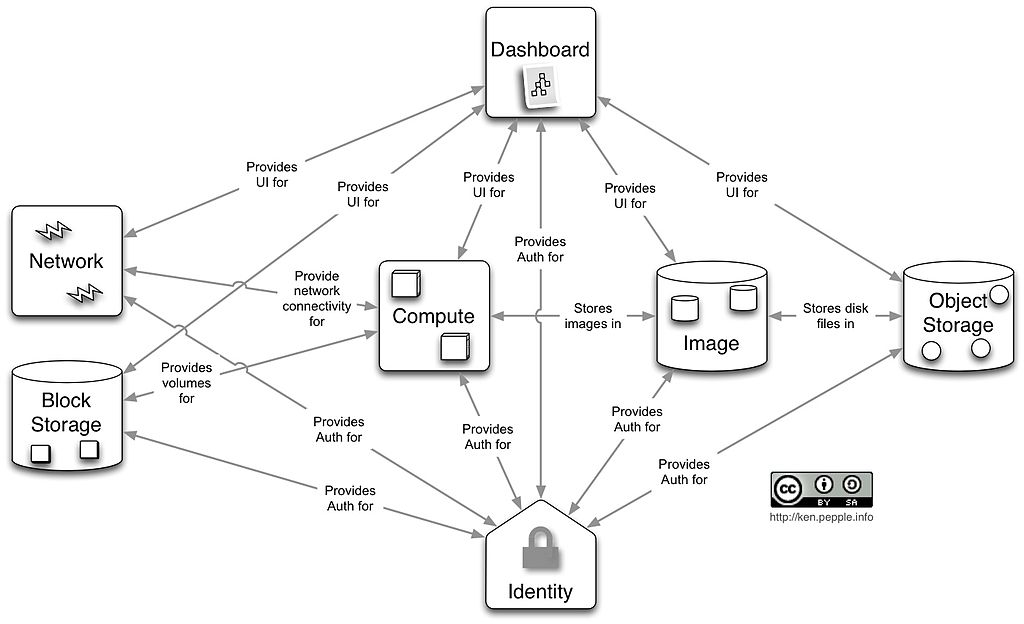
\includegraphics[width=.9\linewidth]{./openstack.jpg}
\end{center}

\section*{VM deployment workflow}
\label{sec:orge1cdd67}
\begin{itemize}
\item Heat engine executes a template
\item Nova schedules VM creation
\item Nova asks Glance for image
\item Glance asks Swift for image contents
\item Heat asks Cinder for volume
\item Nova asks Neutron for network
\end{itemize}

\subsection*{VM deployment workflow}
\label{sec:org1773114}
\begin{center}
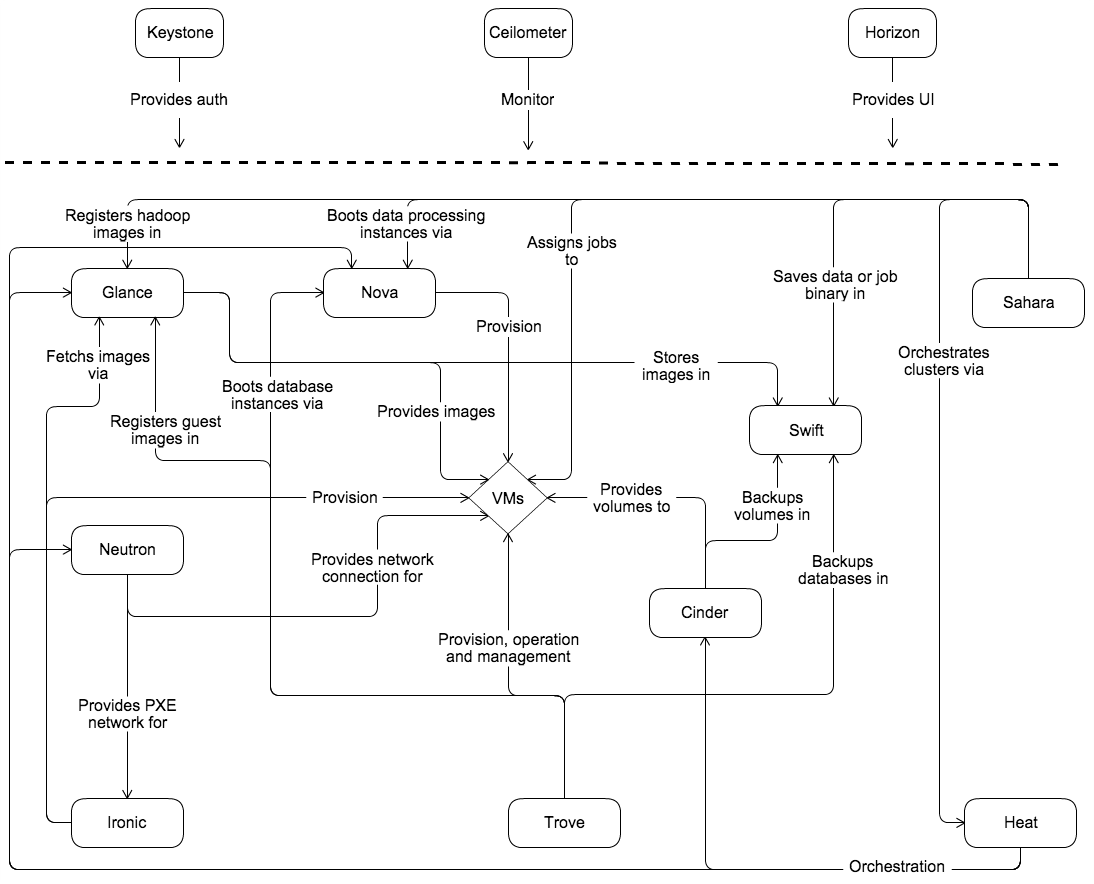
\includegraphics[width=.9\linewidth]{./openstack-conceptual-arch-kilo.png}
\end{center}

\subsection*{VM deployment workflow}
\label{sec:org3ff61f0}
\begin{center}
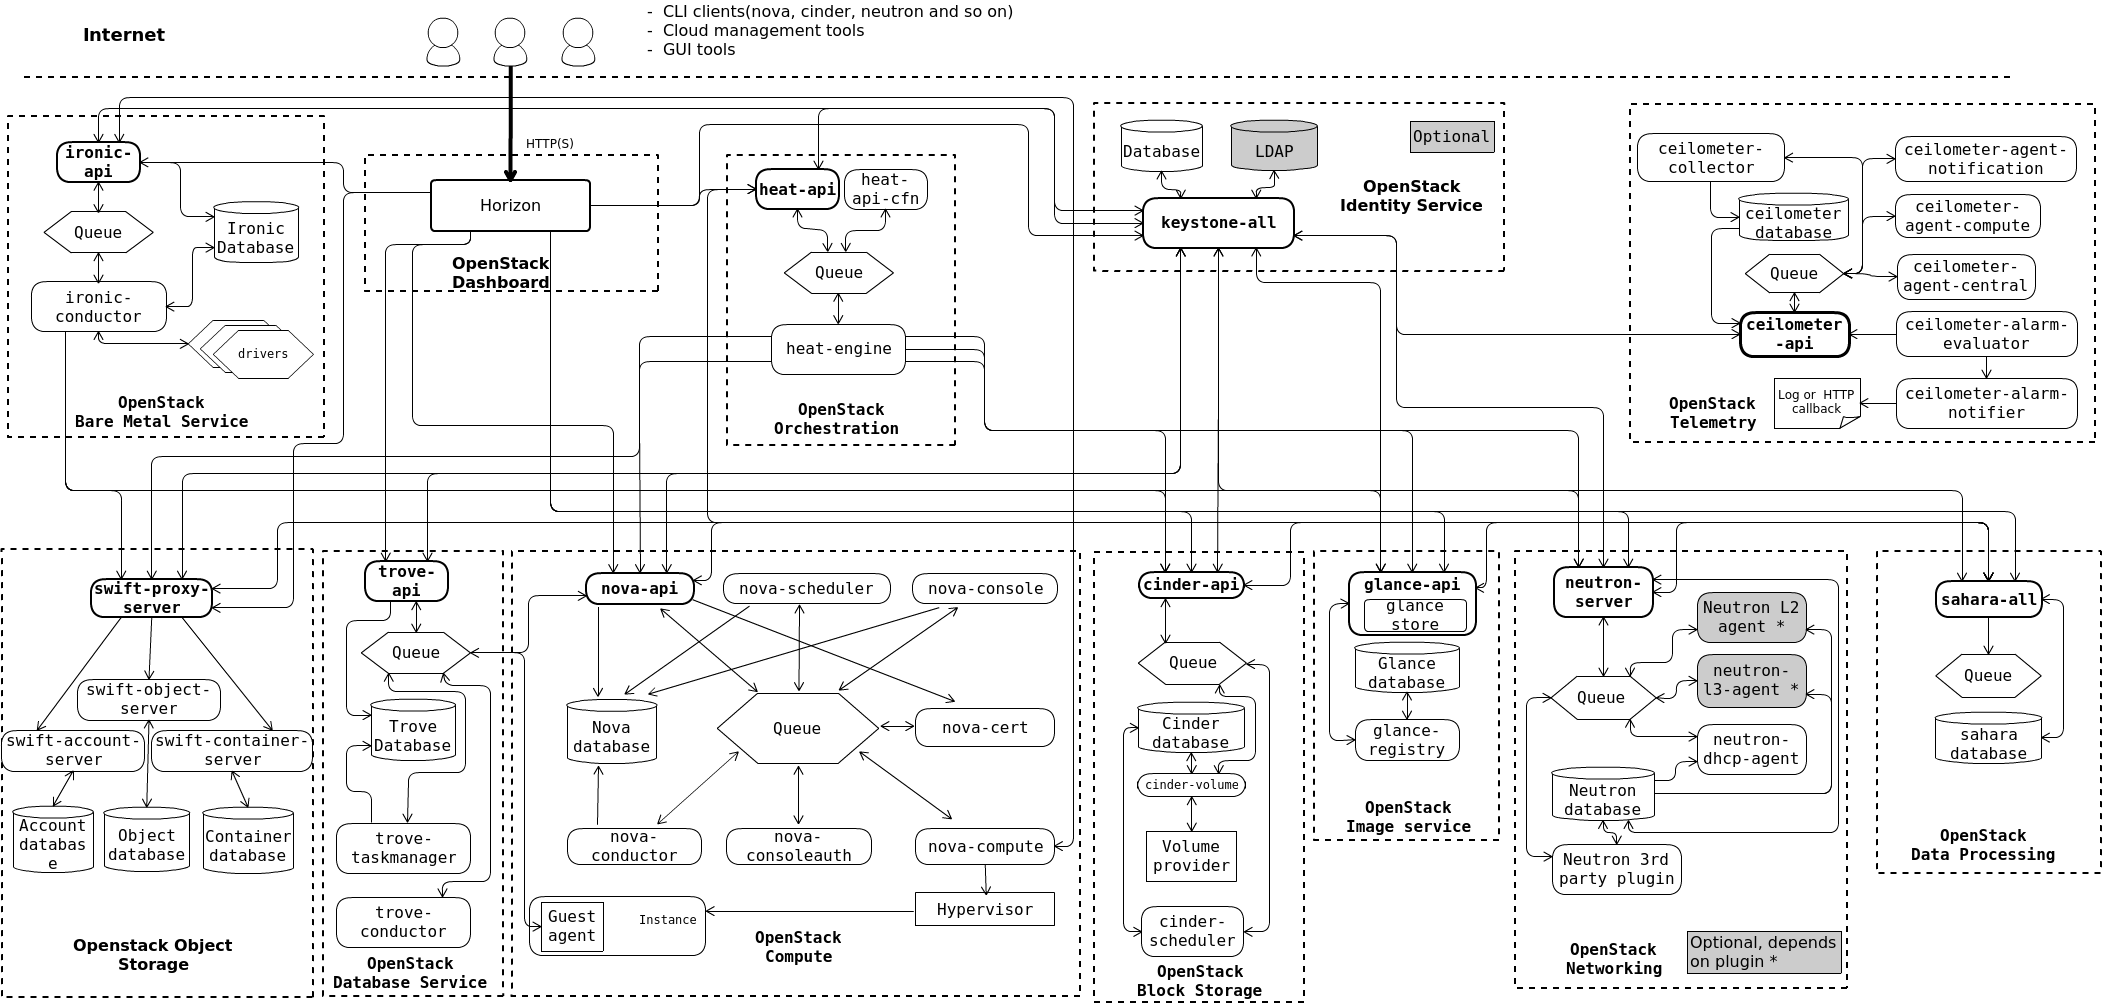
\includegraphics[width=.9\linewidth]{./openstack-logical-arch-kilo.png}
\end{center}

\section*{OpenStack service structure}
\label{sec:orge2943e6}
\begin{itemize}
\item Message queue
\item Persistent database
\item REST API service
\item Service engine
\item Remote agent
\end{itemize}

\section*{Other OpenStack services}
\label{sec:orgee820a1}
\begin{itemize}
\item Orchestration - Heat
\item Baremetal provisioning - Ironic
\item Non/relational database service - Trove
\item Dashboard - Horison
\item Block Storage - Cinder
\item Telemetry - Ceilometer
\end{itemize}

\section*{More OpenStack services}
\label{sec:orge3df3f5}
\begin{itemize}
\item Elastic Map Reduce - Sahara
\item Messaging Service - Zaqar
\item Shared Filesystems - Manila
\item DNS Service - Designate
\item Key Management - Barbican
\item Containers - Magnum
\item Application Catalog - Murano
\item Governance - Congress
\end{itemize}

\section*{OpenStack governance}
\label{sec:orgfaf4906}
\begin{itemize}
\item Open source
\item Open community
\item Open design
\item Open development
\end{itemize}

\section*{Open source}
\label{sec:orga1893ea}
\begin{itemize}
\item Fully functional, no vendor-specifics
\item Apache 2.0 License
\end{itemize}

\section*{Open community}
\label{sec:org1a4e1d4}
\begin{itemize}
\item Public meetings on IRC
\item Mailing lists, bugs on Launchpad and Storyboard
\item Elected Project Team Lead
\item Elected Technical Committee
\end{itemize}

\section*{Open design}
\label{sec:org8084a6b}
\begin{itemize}
\item OpenStack Summit
\item OpenStack Forum
\item Project Team Gatherings
\end{itemize}

\section*{Open development}
\label{sec:org4113318}
\begin{itemize}
\item Code contributions - \url{https://review.openstack.org/}
\item Project Team Lead
\item Core Reviewers
\item Specifications - \url{https://specs.openstack.org/}
\end{itemize}

\section*{Questions?}
\label{sec:org5a9d8e3}
\begin{itemize}
\item \url{https://www.openstack.org/}
\end{itemize}
\end{document}